%\documentclass[12pt,twoside]{article}
\documentclass[conference]{IEEEtran}  % this should work with your LaTeX installation; else download extra package (www.ctan.org/pkg/ieeetran) or remove IEEE usage below

%%%%%%% Fill this out:
\newcommand{\trtitle}{(Fine-tuned BERT) Encoder Comparison for Document Classification}
\newcommand{\titleshort}{KPIS EC4DC} % title for header:
\newcommand{\authorlastnames}{Ebert, Hamza} % alphabetical for seminars
\newcommand{\trcourse}{Knowledge Processing in Intelligent Systems: Practical Seminar}
\newcommand{\trgroup}{Knowledge Technology, WTM}
\newcommand{\truniversity}{Department of Informatics, University of Hamburg}
%%%%%%%%%%%%%%%%%%%%%%%%%%%%%%%%%%%%%%%%%%%%%%%%%%%%%%%%%%%%%
% Languages:

% If the thesis is written in English:
\usepackage[english]{babel} 						
\selectlanguage{english}

%%%%%%%%%%%%%%%%%%%%%%%%%%%%%%%%%%%%%%%%%%%%%%%%%%%%%%%%%%%%%
% Bind packages:

\usepackage{acronym}                    % Acronyms
\usepackage{algorithmic}				% Algorithms and Pseudocode
\usepackage{algorithm}				% Algorithms and Pseudocode
\usepackage{amsfonts}                   % AMS Math Packet (Fonts)
\usepackage{amsmath}                    % AMS Math Packet
\usepackage{amssymb}                    % Additional mathematical symbols
\usepackage{amsthm}
\usepackage{booktabs}
\usepackage{tikz}
\definecolor{newgreen}{rgb}{0.0,0.5,0.15}
\newcommand{\new}[1]{\textcolor{newgreen}{#1}}  % new since the pushed outline, remove before submitting
\usetikzlibrary{calc}                   % Nicer tables
%\usepackage[font=small,labelfont=bf]{caption} % Numbered captions for figures
\usepackage{color}                      % Enables defining of colors via \definecolor
\definecolor{uhhRed}{RGB}{254,0,0}		  % Official Uni Hamburg Red
\definecolor{uhhGrey}{RGB}{122,122,120} % Official Uni Hamburg Grey
\usepackage{fancybox}                   % Gleichungen einrahmen
\usepackage{fancyhdr}					% Packet for nicer headers
%\usepackage{fancyheadings}             % Nicer numbering of headlines

%\usepackage[outer=3.35cm]{geometry} 	  % Type area (size, margins...) !!!Release version
%\usepackage[outer=2.5cm]{geometry} 		% Type area (size, margins...) !!!Print version
%\usepackage{geometry} 					% Type area (size, margins...) !!!Proofread version
\usepackage{geometry} 	  % Type area (size, margins...) !!!Draft version
\geometry{a4paper,body={7.0in,9.1in}}

\usepackage{graphicx}                   % Inclusion of graphics
%\usepackage{latexsym}                  % Special symbols
\usepackage{longtable}				% Allow tables over several parges
\usepackage{listings}                   % Nicer source code listings
\usepackage{multicol}					% Content of a table over several columns
\usepackage{multirow}					% Content of a table over several rows
\usepackage{rotating}					% Alows to rotate text and objects
%\usepackage[hang]{subfigure}            % Allows to use multiple (partial) figures in a fig
%\usepackage[font=footnotesize,labelfont=rm]{subfig}	% Pictures in a floating environment
\usepackage{tabularx}					% Tables with fixed width but variable rows
\usepackage{url,xspace,boxedminipage}   % Accurate display of URLs

%%%%%%%%%%%%%%%%%%%%%%%%%%%%%%%%%%%%%%%%%%%%%%%%%%%%%%%%%%%%%
% Configurationen:

\hyphenation{whe-ther} 				% Manually use: "\-" in a word: Staats\-ver\-trag

%\lstloadlanguages{C}                   % Set the default language for listings
\DeclareGraphicsExtensions{.pdf,.svg,.jpg,.png,.eps} % first try pdf, then eps, png and jpg
\graphicspath{{./src/}} 				% Path to a folder where all pictures are located
\pagestyle{fancy} 					% Use nicer header and footer

% Redefine the environments for floating objects:
\setcounter{topnumber}{3}
\setcounter{bottomnumber}{2}
\setcounter{totalnumber}{4}
\renewcommand{\topfraction}{0.9} 			  %Standard: 0.7
\renewcommand{\bottomfraction}{0.5}		  %Standard: 0.3
\renewcommand{\textfraction}{0.1}		  	%Standard: 0.2
\renewcommand{\floatpagefraction}{0.8} 	%Standard: 0.5

% Tables with a nicer padding:
\renewcommand{\arraystretch}{1.2}

%%%%%%%%%%%%%%%%%%%%%%%%%%%%
% Additional 'theorem' and 'definition' blocks:
\theoremstyle{plain}
\newtheorem{theorem}{Theorem}[section]
%\newtheorem{theorem}{Satz}[section]		% Wenn in Deutsch geschrieben wird.
\newtheorem{axiom}{Axiom}[section] 	
%\newtheorem{axiom}{Fakt}[chapter]		% Wenn in Deutsch geschrieben wird.
%Usage:%\begin{axiom}[optional description]%Main part%\end{fakt}

\theoremstyle{definition}
\newtheorem{definition}{Definition}[section]

%Additional types of axioms:
\newtheorem{lemma}[axiom]{Lemma}
\newtheorem{observation}[axiom]{Observation}

%Additional types of definitions:
\theoremstyle{remark}
%\newtheorem{remark}[definition]{Bemerkung} % Wenn in Deutsch geschrieben wird.
\newtheorem{remark}[definition]{Remark} 

%%%%%%%%%%%%%%%%%%%%%%%%%%%%
% Provides TODOs within the margin:
\newcommand{\TODO}[1]{\marginpar{\emph{\small{{\bf TODO: } #1}}}}

%%%%%%%%%%%%%%%%%%%%%%%%%%%%
% Abbreviations and mathematical symbols
\newcommand{\modd}{\text{ mod }}
\newcommand{\RS}{\mathbb{R}}
\newcommand{\NS}{\mathbb{N}}
\newcommand{\ZS}{\mathbb{Z}}
\newcommand{\dnormal}{\mathit{N}}
\newcommand{\duniform}{\mathit{U}}

\newcommand{\erdos}{Erd\H{o}s}
\newcommand{\renyi}{-R\'{e}nyi}
\usepackage{graphicx}

% correct bad hyphenation here
\hyphenation{}

%%%%%%%%%%%%%%%%%%%%%%%%%%%%%%%%%%%%%%%%%%%%%%%%%%%%%%%%%%%%%
% Document:
\begin{document}

\title{\trtitle\\[1.5ex]
\large \trcourse\\[0.5ex]
\trgroup\\[0.5ex]
\truniversity}

\renewcommand{\headheight}{14.5pt}
\fancyhead[LO]{\slshape \authorlastnames}
\fancyhead[RO]{ \slshape \titleshort}

\author{\IEEEauthorblockN{Sabrina Ebert}
\IEEEauthorblockA{\textit{sabrina.ebert@studium.uni-hamburg.de}}
\and
\IEEEauthorblockN{Muhammad Hamza}
\IEEEauthorblockA{\textit{muhammad.hamza-2@studium.uni-hamburg.de}}
}

\maketitle

% Outline (assignment 3): 4 pages + appendix

\begin{abstract}
Encoder models like BERT are small and cheap compared to large language models and are often used for classifying texts.
LoRA makes fine-tuning them cheaper by training only a few small added matrices.
It comes with several settings, such as rank, learning rate and which layers it is added to, and it is not clear to us which of them matter most for a small encoder.
In this work we fine-tune BERT-base with LoRA for \new{classifying sentences, short news texts and full documents (SST-2, AG News, 20 Newsgroups)} and measure if and for which settings the classification performance changes, and by how much.
We change one setting at a time, run every setting with three seeds and compare accuracy and macro F1 to a frozen BERT baseline.
Our working hypothesis is that learning rate and LoRA placement change the performance more than the rank does.
If time allows, we also take a first look inside the fine-tuned models with explainable AI methods, e.g.\ word attributions, to explain the results.
\end{abstract}

\IEEEpeerreviewmaketitle

\section{Introduction and Motivation}
\label{sec:introduction}
\begin{itemize}
  \item encoders small and cheap vs.\ LLMs
  \item LoRA: many settings, little guidance
\end{itemize}

\section{Theoretical Background}
\label{sec:background}
\subsection{BERT}
\subsection{LoRA}
\new{Fine-tuning changes a weight matrix $W_0 \in \mathbb{R}^{d \times k}$ into $W_0 + \Delta W$.}
\new{LoRA assumes that this change needs only a few directions, a low ``intrinsic rank'', and writes it as the product of two thin matrices \cite{hu2022lora}:}
\begin{equation}
  \color{newgreen} h = W_0 x + \tfrac{\alpha}{r} B A x, \quad B \in \mathbb{R}^{d \times r},\ A \in \mathbb{R}^{r \times k},\ r \ll \min(d, k).
\end{equation}
\new{$W_0$ stays frozen, only $A$ and $B$ are trained (Fig.~\ref{fig:lora}).}
\new{$A$ starts random and $B$ at zero, so training starts exactly from the pretrained model.}
\new{$\alpha / r$ scales the update. Hu et al.\ set $\alpha$ once and do not tune it \cite[Sec.~4.1]{hu2022lora}.}
\new{After training, $BA$ can be added to $W_0$, so the model is as fast as before.}

\new{The rank $r$ is the number of independent patterns the update can hold: $BA = \sum_{j=1}^{r} b_j a_j^\top$, one column of $B$ times one row of $A$ each (Fig.~\ref{fig:rank}).}
\new{With $r = 1$, every row of $\Delta W$ is a multiple of the same row $a_1^\top$, so the weights can only change along one direction.}
\new{For one $768 \times 768$ attention matrix of BERT-base \cite{devlin2019bert} and $r = 8$, LoRA trains $2 \cdot 768 \cdot 8 = 12{,}288$ instead of $589{,}824$ weights, about 2\%.}
\new{With LoRA on query and value in all 12 layers plus the classification layer, 296,450 weights are trained, 0.27\% of the model.}
\new{What is left to choose: the rank $r$, the scale $\alpha$, which matrices and which layers get LoRA, and the usual training settings.}

\new{\textit{Which layers.} Lower BERT layers encode word types and syntax, higher layers semantic relations such as roles and coreference \cite[Sec.~4]{tenney2019pipeline}.}
\new{Fine-tuning changes mostly the top layers, and freezing all but the last few costs little \cite[Sec.~5]{merchant2020happens}.}
\new{For classification the last layer gives the best features \cite[Tab.~3]{sun2019finetune}.}
\new{So LoRA can be restricted to the last blocks, e.g.\ layers 10--12 (\texttt{layers\_to\_transform=[9,10,11]}), which trains 75,266 instead of 296,450 weights at $r = 8$.}
\new{At the same budget, top layers clearly beat bottom layers \cite[Fig.~1b]{zhang2023adalora}.}
\new{Which layers are needed depends on the task \cite{zuo2026layer}, so we test it.}

\begin{figure}[t]
\new{\centering}
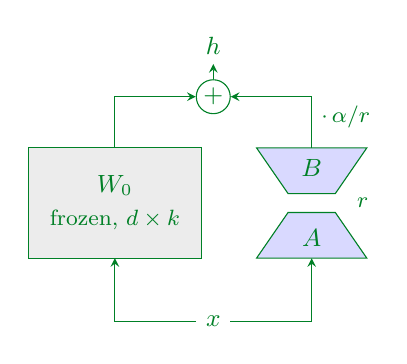
\begin{tikzpicture}[font=\small, >=stealth]
\new{  \draw[fill=gray!15] (-1.1,-0.7) rectangle (1.1,0.7);}
\new{  \node[align=center] at (0,0) {$W_0$\\[1pt]\footnotesize frozen, $d \times k$};}
\new{  \draw[fill=blue!15] (1.8,-0.7) -- (3.2,-0.7) -- (2.8,-0.12) -- (2.2,-0.12) -- cycle;}
\new{  \draw[fill=blue!15] (2.2,0.12) -- (2.8,0.12) -- (3.2,0.7) -- (1.8,0.7) -- cycle;}
\new{  \node at (2.5,-0.45) {$A$};}
\new{  \node at (2.5,0.45) {$B$};}
\new{  \node[font=\footnotesize] at (3.15,0) {$r$};}
\new{  \node (x) at (1.25,-1.5) {$x$};}
\new{  \node[draw, circle, inner sep=1pt] (plus) at (1.25,1.35) {$+$};}
\new{  \node (h) at (1.25,2.0) {$h$};}
\new{  \draw[->] (x) -| (0,-0.7);}
\new{  \draw[->] (x) -| (2.5,-0.7);}
\new{  \draw[->] (0,0.7) |- (plus);}
\new{  \draw[->] (2.5,0.7) |- node[pos=0.3, right, font=\footnotesize] {$\cdot\,\alpha / r$} (plus);}
\new{  \draw[->] (plus) -- (h);}
\end{tikzpicture}
\caption{\new{LoRA: the frozen weight $W_0$ gets a trainable low-rank path $BA$ next to it. Only the blue part is trained. After \cite{hu2022lora}, Fig.~1.}}
\label{fig:lora}
\end{figure}

\begin{figure}[t]
\centering
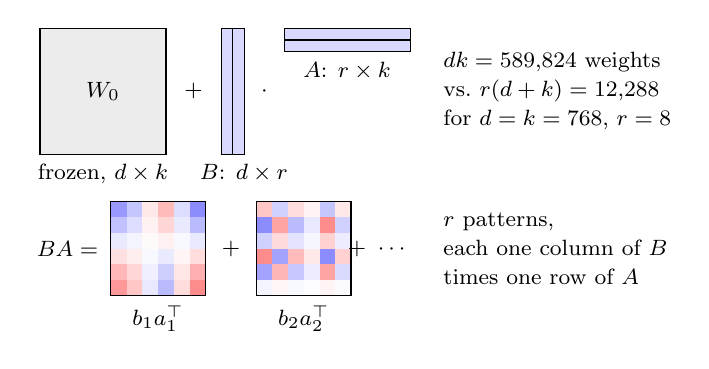
\begin{tikzpicture}[font=\footnotesize]
  % row 1: W0 + B A
  \draw[fill=gray!15] (0,0) rectangle (1.6,1.6); \node at (0.8,0.8) {$W_0$};
  \node[below] at (0.8,0) {frozen, $d \times k$};
  \node at (1.95,0.8) {$+$};
  \draw[fill=blue!15] (2.3,0) rectangle (2.6,1.6); \draw (2.45,0) -- (2.45,1.6);
  \node[below, xshift=4pt] at (2.45,0) {$B$: $d \times r$};
  \node at (2.85,0.8) {$\cdot$};
  \draw[fill=blue!15] (3.1,1.3) rectangle (4.7,1.6); \draw (3.1,1.45) -- (4.7,1.45);
  \node[below] at (3.9,1.3) {$A$: $r \times k$};
  \node[align=left, anchor=west] at (5.0,0.8) {$d k = 589{,}824$ weights\\[1pt]vs.\ $r(d + k) = 12{,}288$\\[1pt]for $d = k = 768$, $r = 8$};
  % row 2: B A as a sum of r patterns
  \node at (0.35,-1.2) {$BA =$};
  \foreach \x/\b/\a/\name in {0.9/{1,0.6,0.2,-0.3,-0.7,-1}/{0.9,0.5,-0.2,-0.6,0.3,1}/{b_1 a_1^\top}, 2.75/{-0.5,1,0.4,-1,0.8,0.1}/{1,-0.8,0.6,0.2,-1,0.4}/{b_2 a_2^\top}} {
    \foreach \i in {0,...,5} {
      \foreach \j in {0,...,5} {
        \pgfmathsetmacro\v{{\b}[\i]*{\a}[\j]}
        \pgfmathsetmacro\o{0.45*abs(\v)}
        \ifdim\v pt>0pt \fill[blue, opacity=\o] (\x+0.2*\j,-0.6-0.2*\i) rectangle ++(0.2,-0.2);
        \else \fill[red, opacity=\o] (\x+0.2*\j,-0.6-0.2*\i) rectangle ++(0.2,-0.2); \fi
      }
    }
    \draw (\x,-0.6) rectangle ++(1.2,-1.2);
    \node[below] at (\x+0.6,-1.8) {$\name$};
  }
  \node at (2.425,-1.2) {$+$};
  \node at (4.3,-1.2) {$+ \ \cdots$};
  \node[align=left, anchor=west] at (5.0,-1.2) {$r$ patterns,\\[1pt]each one column of $B$\\[1pt]times one row of $A$};
\end{tikzpicture}
\caption{\new{The LoRA update as matrices. Top: the frozen $W_0$ gets $BA$ added, two thin matrices with $r$ columns and rows. Bottom: $BA$ is a sum of $r$ simple patterns. Each pattern changes every row of $W_0$ in the same direction, only scaled (blue = up, red = down). A higher rank allows more different directions.}}
\label{fig:rank}
\end{figure}

\subsection{Related Work}

\section{Experimental Setup}
\label{sec:setup}
\begin{itemize}
  \item Kaggle, SST-2, AG News\new{, 20 Newsgroups}
  \item baseline, LoRA study, \new{other datasets}
  \item libraries: transformers, peft, scikit-learn, maybe captum (XAI)
  \item 3 seeds per setting
\end{itemize}

\subsection{\new{Datasets}}
\new{Three datasets, from single sentences to whole documents (Fig.~\ref{fig:datasets}). Dev is used for all choices, test is scored once at the end.}
\begin{itemize}
  \item \new{GLUE: benchmark of 9 English sentence tasks, test labels are hidden and scored on a server \cite{wang2019glue}. We use one task, SST-2.}
  \item \new{SST-2: movie review sentences, positive or negative \cite{socher2013sst}. Train has 67,349 items, mostly short phrases cut out of sentences (median 7 words), validation 872 full sentences. We split validation into dev and test.}
  \item \new{AG News: news title and description, 4 topics (world, sports, business, science and technology), 30,000 train and 1,900 test texts per topic \cite{zhang2015charcnn}. Median 50 tokens, under 1\% longer than 128.}
  \item \new{20 Newsgroups: forum posts from 20 groups, 11,314 train and 7,532 test, mail headers removed \cite{lang1995newsweeder}. Median 132 tokens, half longer than 128, 9\% longer than 512, so text length matters here.}
\end{itemize}

\begin{figure}[t]
\centering
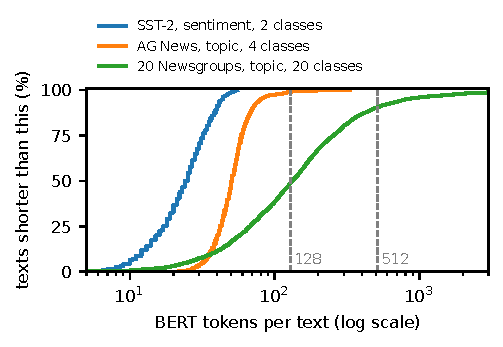
\includegraphics[width=\columnwidth]{fig_datasets.pdf}
\caption{\new{Text length of the three datasets: SST-2 sentences (validation), AG News and 20 Newsgroups (3000 random training texts each). AG News stays below 128 tokens, half of the 20 Newsgroups posts are longer, about one in ten longer than 512.}}
\label{fig:datasets}
\end{figure}

\subsection{\new{Classifier on top}}
\new{BERT gives one vector of 768 numbers per token. A class needs one vector per text: the [CLS] vector or the mean over all tokens.}
\new{A linear layer turns it into one score per class, softmax into probabilities, and cross entropy is the loss \cite{devlin2019bert}.}
\begin{itemize}
  \item \new{baseline: BERT frozen, only a logistic regression on the mean vector is trained}
  \item \new{LoRA: the linear layer is trained together with LoRA in the chosen layers, all BERT weights stay frozen (Fig.~\ref{fig:setup})}
  \item \new{weights that change, $r = 8$ on query + value, 2 classes: $294{,}912$ LoRA + $1{,}538$ classifier}
  \item \new{Hugging Face's classifier first passes [CLS] through BERT's pretrained pooler layer, which stays frozen}
\end{itemize}

\begin{figure}[t]
\centering
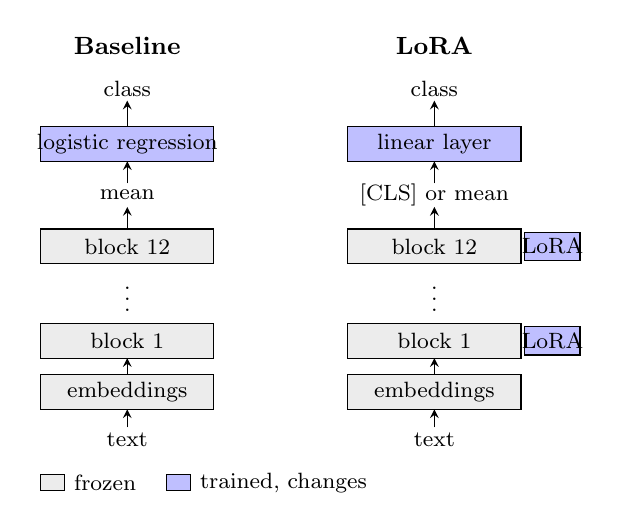
\begin{tikzpicture}[font=\footnotesize, >=stealth]
  \foreach \x/\title/\pool/\head/\lora in {0/Baseline/mean/logistic regression/0, 3.9/LoRA/{[CLS] or mean}/linear layer/1} {
    \node[font=\small\bfseries] at (\x+1.1,5.0) {\title};
    \node at (\x+1.1,0) {text};
    \foreach \y/\name in {0.6/embeddings, 1.25/block 1, 2.45/block 12} {
      \draw[fill=gray!15] (\x,\y-0.22) rectangle (\x+2.2,\y+0.22);
      \node at (\x+1.1,\y) {\name};
    }
    \node at (\x+1.1,1.88) {$\vdots$};
    \ifnum\lora=1
      \foreach \y in {1.25, 2.45} {
        \draw[fill=blue!25] (\x+2.25,\y-0.18) rectangle (\x+2.95,\y+0.18);
        \node at (\x+2.6,\y) {LoRA};
      }
    \fi
    \node at (\x+1.1,3.1) {\pool};
    \draw[fill=blue!25] (\x,3.53) rectangle (\x+2.2,3.97);
    \node at (\x+1.1,3.75) {\head};
    \node at (\x+1.1,4.45) {class};
    \foreach \a/\b in {0.15/0.38, 0.82/1.03, 2.67/2.95, 3.25/3.53, 3.97/4.3} {
      \draw[->] (\x+1.1,\a) -- (\x+1.1,\b);
    }
  }
  \draw[fill=gray!15] (0,-0.65) rectangle (0.3,-0.45); \node[right] at (0.3,-0.55) {frozen};
  \draw[fill=blue!25] (1.6,-0.65) rectangle (1.9,-0.45); \node[right] at (1.9,-0.55) {trained, changes};
\end{tikzpicture}
\caption{\new{The two setups. Grey parts stay as pretrained, only blue parts change during training. LoRA layers and modules are the settings we vary.}}
\label{fig:setup}
\end{figure}

\subsection{\new{Metrics}}
\new{For $N$ dev texts with true class $y_i$, the predicted class is $\hat y_i = \arg\max_c (W v_i + b)_c$, trained with cross entropy.}
\begin{equation}
  \color{newgreen} \text{acc} = \frac{1}{N} \sum_{i=1}^{N} [\hat y_i = y_i], \qquad
  R_c = \frac{\#\{\hat y_i = y_i = c\}}{\#\{y_i = c\}}
\end{equation}
\new{$R_c$ is the accuracy within class $c$, $P_c$ the same among texts predicted as $c$.}
\new{Macro F1 averages $F1_c = 2 P_c R_c / (P_c + R_c)$ over the $C$ classes, so small classes count as much as large ones.}
\new{Every value is the mean over 3 seeds, changes are given in points against the reference.}

\subsection{\new{Settings to try, from earlier work}}
\new{Sorted from where LoRA sits to how it is trained. Values are the ones reported, mostly for other models.}
\begin{itemize}
  \item \new{layers: LoRA only in layers 10--12 nearly as good as all, only 1--3 much worse, 88.60 vs.\ 77.87 on MNLI-m, same budget, DeBERTaV3-base \cite[Fig.~1b]{zhang2023adalora}}
  \item \new{layers: full fine-tuning with all but the top layers frozen keeps most of the accuracy \cite[Sec.~5.2]{merchant2020happens}}
  \item \new{layers: about 30\% of the layers enough, which ones depends on the task, decoder \cite{zuo2026layer}}
  \item \new{modules: feed-forward 89.99 vs.\ query only 88.58, MNLI-m, same budget \cite[Fig.~1a]{zhang2023adalora}}
  \item \new{modules: query + value better than one matrix with higher rank, all four attention matrices best on MNLI, 91.7, GPT-3 \cite[Tab.~5]{hu2022lora}}
  \item \new{modules: all matrices better than two on all 8 GLUE tasks, on SST-2 only by 0.11 \cite[Tab.~14]{zhang2023adalora}}
  \item \new{modules: all attention vs.\ query + value at $r = 8$: 59.2 vs.\ 53.4 exact match, T5-small \cite{rathor2026howsmall}}
  \item \new{rank: $r = 1$ to $64$ on query + value within 0.5 points, GPT-3 \cite[Tab.~6]{hu2022lora}}
  \item \new{rank: $r = 2$ and $r = 8$ both 94.95 on SST-2, DeBERTaV3-base \cite[Tab.~1]{zhang2023adalora}}
  \item \new{rank: $r = 8$ vs.\ $32$ on SST-2: 93.46 vs.\ 93.58, RoBERTa-base \cite{li2025tokenwise}}
  \item \new{rank: no gain from higher rank on a small BERT, rank 1 almost no loss \cite[Sec.~4.4]{frees2025lora}}
  \item \new{rank: only very small budgets lose, SST-2 94.38 at 0.08\% vs.\ 94.95 at 0.16\% of the weights \cite[Tab.~5]{zhang2023adalora}}
  \item \new{alpha: $\alpha = 2r$ common, e.g.\ 16 for $r = 8$ \cite[Tab.~9]{hu2022lora}, set once and not tuned \cite[Sec.~4.1]{hu2022lora}}
  \item \new{learning rate: $4\cdot10^{-4}$ to $5\cdot10^{-4}$ on GLUE, $5\cdot10^{-4}$ on SST-2, RoBERTa-base \cite[Tab.~9]{hu2022lora}, far above $2\cdot10^{-5}$ to $5\cdot10^{-5}$ for full fine-tuning \cite{devlin2019bert}}
  \item \new{learning rate: most sensitive setting, Llama-3.1-8B \cite{he2026unified}}
  \item \new{training: batch 16, warmup 6\%, 60 epochs on SST-2, RoBERTa-base \cite[Tab.~9]{hu2022lora}}
  \item \new{pooling: mean better than [CLS] for frozen BERT \cite[Tab.~1]{ma2019universal}, no results with LoRA found}
  \item \new{text length: last 510 tokens better than first, IMDb test error 5.44 vs.\ 5.63, head + tail 5.42 \cite[Tab.~2]{sun2019finetune}}
\end{itemize}

\section{Results}
\label{sec:results}

\section{Discussion and Outlook}
\label{sec:discussion}

\section*{Acknowledgments and Use of Tools and AI}
We used Claude Code (Anthropic) to set up the LaTeX layout, to suggest some of the references to draft the abstract from our milestones, \new{to draft the LoRA and classifier sections with their sketches and the list of settings from the cited papers,} and to improve grammar and wording.
The topic, study design and working hypothesis are our own.
We checked all text and references and take full responsibility for the content.

\nocite{devlin2019bert,hu2022lora,sun2019finetune,dodge2020finetuning,socher2013sst,wang2019glue,zhang2015charcnn,lang1995newsweeder}

\clearpage
\bibliographystyle{plain}
\bibliography{bib}

\section*{Appendix: Code}

\end{document}
